Modify the RBF interpolation to include a polynomial correction. In 2D, this amounts to searching for an interpolant of
the form

$$
F(\bm{x}) = \sum\limits_{j=1}^N c_j \phi\left( \lVert \bm{x} - \bm{x}_j \rVert \right) + p(\bm{x})
$$

where $p(\bm{x}) = p(x, y) = \gamma_1 + \gamma_2 x + \gamma_3 y$.

\begin{solution}
    To implement a polynomial correction, we introduce the following modified linear system to solve for the polynomial 
    coefficients $\gamma_i$ (where $A$ is as in Problem 1):

    $$
    \begin{pmatrix}
          &       &     & | & 1 & x_1    & y_1    \\
          & A     &     & | & 1 & \vdots & \vdots \\
          &       &     & | & 1 & x_n    & y_n    \\
        - & -     &   - & + & - & -      & -      \\
        1 & \dots &   1 & | &   &        &        \\
      x_1 & \dots & x_n & | &   & 0      &        \\
      y_1 & \dots & y_n & | &   &        &        \\
    \end{pmatrix} \begin{pmatrix}
      c_1 \\
      \vdots \\
      c_n \\
      - \\
      \gamma_1 \\
      \gamma_2 \\
      \gamma_3 \\
    \end{pmatrix} = \begin{pmatrix}
      f_1 \\
      \vdots \\
      f_n \\
      - \\
      0 \\
      0 \\
      0
    \end{pmatrix}
    $$

    where we have imposed the constraints 
    $\sum\limits_{k=1}^n c_k = \sum\limits_{k=1}^n c_k x_k = \sum\limits_{k=1}^n c_k y_k = 0$.

    Upon solving for these coefficients for the squircle formulated in Problem 1 in \texttt{problem\_2i.m}, we obtain 
    the following values for $\gamma_i$:

    $$
        \gamma_1 = 1.1755, \quad \gamma_2 = 0.022566, \quad \text{and} \quad \gamma_3 = -2.0023581 \\
    $$
   
    We plot the resulting interpolation in Figure \ref{fig:problem_2i}.
    \begin{figure}[h]
        \centering
        \begin{subfigure}{0.49\textwidth}
            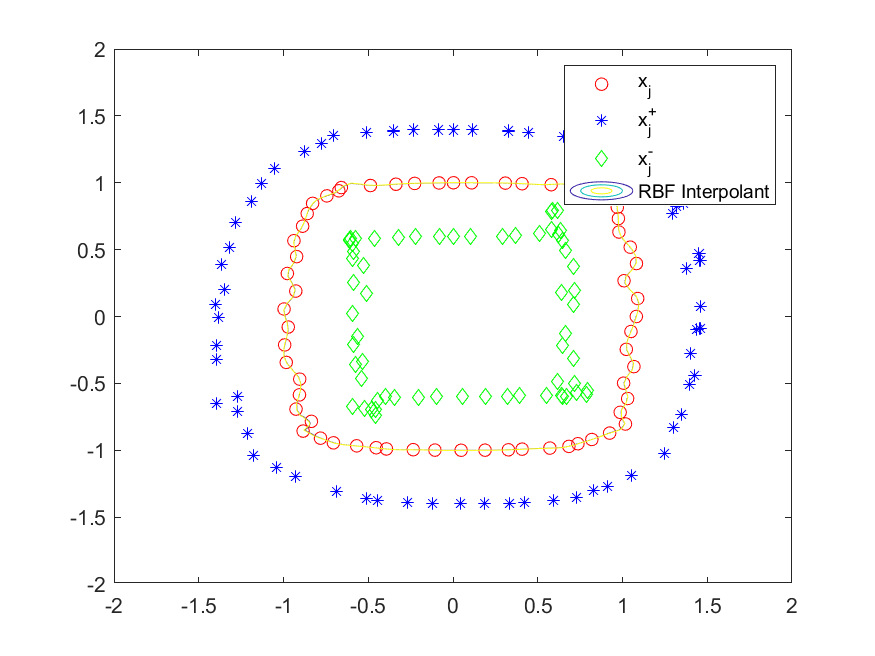
\includegraphics[width=\textwidth]{problem_2i_interpolant_2d.png}
            \caption{RBF interpolation of source point cloud}
            \label{fig:problem_2i_interpolant_2d}
        \end{subfigure}
        \begin{subfigure}{0.49\textwidth}
            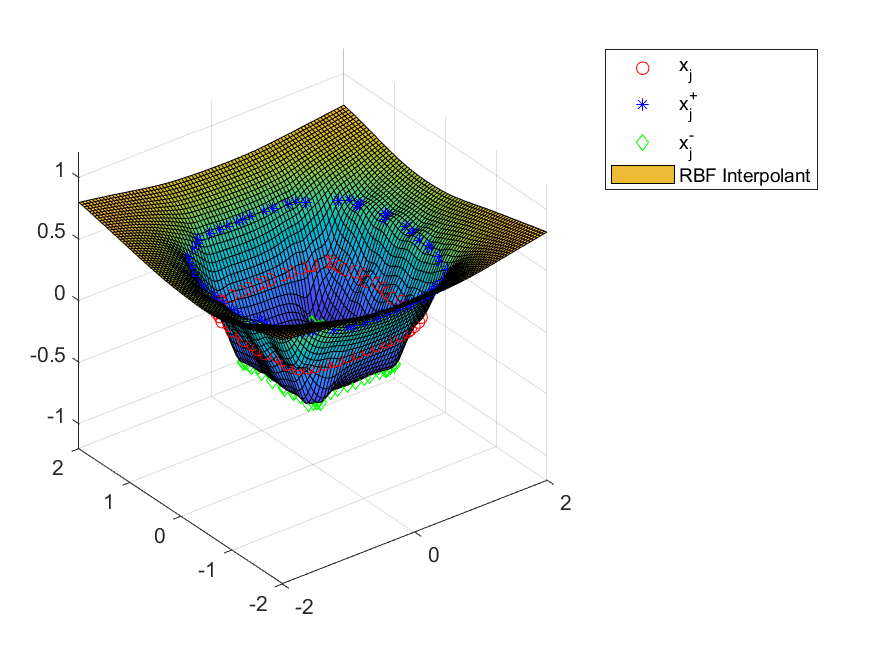
\includegraphics[width=\textwidth]{problem_2i_interpolant_3d.png}
            \caption{3D interpolant of normal point cloud}
            \label{fig:problem_2i_interpolant_3d}
        \end{subfigure}
        \caption{RBF interpolation with polynomial correction}
        \label{fig:problem_2i}
    \end{figure}
\end{solution}